
%(BEGIN_QUESTION)
% Copyright 2014, Tony R. Kuphaldt, released under the Creative Commons Attribution License (v 1.0)
% This means you may do almost anything with this work of mine, so long as you give me proper credit

Denne gassbrenneren gjør giftige gassstrømmer mindre farlige ved høytemperatur forbrenning:

$$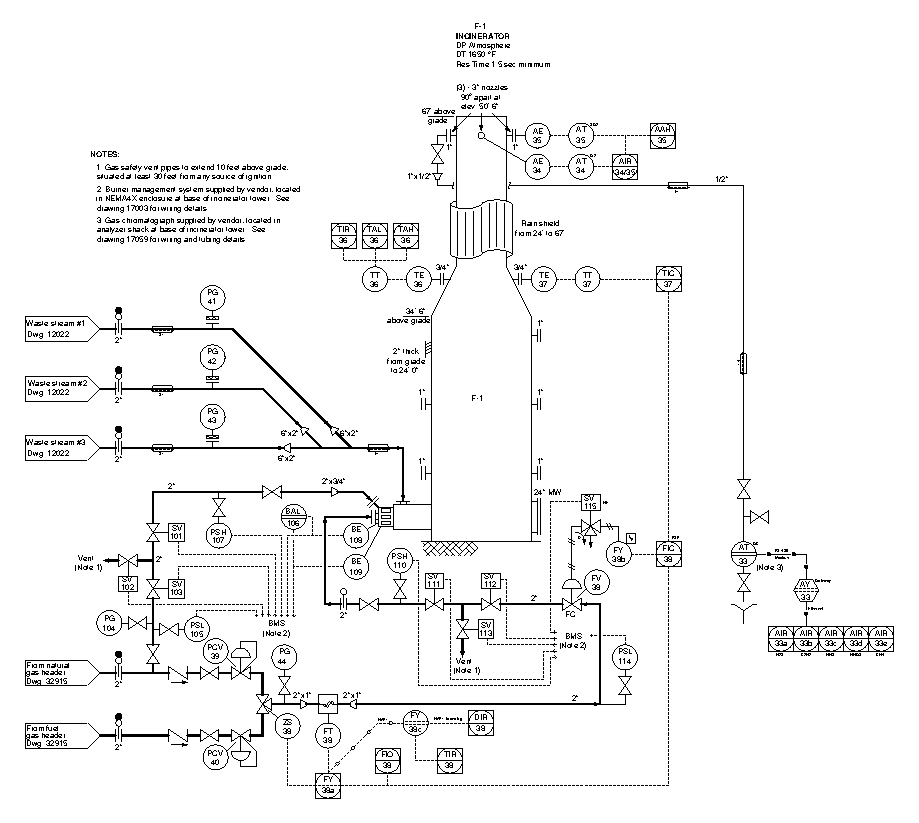
\includegraphics[width=15.5cm]{i0004rx01.eps}$$

Røykgassanalyzer AT-35 måler SO$_2$ via optisk fluorescens. Hvis høyspenningsforsyningen til fotomultiplikatoren i AT-35 feiler til 0 V, hvordan påvirkes AT-35-signalet?

\vskip 10pt

Hvis termoelement TE-37 kortslutter i terminalblokken, hvordan påvirker dette forbrenningens effektivitet og risiko for uoksiderte giftgasser?

\vskip 10pt

Hvis brenngassen får høyere tetthet ($\rho$) og høyere spesifikk varme ($c$), vil FT-38 vise for høyt, for lavt, eller fortsatt korrekt?

\underbar{file i00964}
%(END_QUESTION)





%(BEGIN_ANSWER)

4 poeng for AT-35, 3 poeng for TE-37, 3 poeng for FT-38.

\vskip 10pt

Lav HV-forsyning i AT-35 gjør at fotomultiplikatoren slutter å virke, og analysatoren vil i praksis vise null SO$_2$.

\vskip 10pt

Kortsluttet TE-37 vil få TT-37 til å lese omgivelsestemperatur, slik at brannreguleringen øker brenngass og gir varmere flamme. Dette gir normalt ikke risiko for uoksiderte giftgasser på samme måte som flammeutfall.

\vskip 10pt

FT-38 vil fortsatt måle korrekt fordi det er en Coriolis sann-masseflowmåler.

%(END_ANSWER)





%(BEGIN_NOTES)

{\bf Denne oppgaven er ment kun for eksamen, ikke for arbeidsark!}.

%(END_NOTES)

